\documentclass[14pt, letterpaper, fleqn]{extarticle}
\linespread{1.2}

%dependencies
\usepackage{graphicx}
\usepackage{amsmath}
\usepackage{amssymb}
\usepackage{wrapfig}
\usepackage{geometry}
\usepackage{float}

\geometry{
	 a4paper,
	 total={170mm,257mm},
	 left=20mm,
	 top=20mm
 }
\graphicspath{ {./images/} }

\newcommand{\RomanNumeralCaps}[1]
    {\MakeUppercase{\romannumeral #1}}

\begin{document}
\begin{titlepage}
   \begin{center}
       \vspace*{2.5cm}

       \textbf{Essential Mathematics for AI}

       \vspace{0.5cm}
        Solving the systems of linear equations
            
       \vspace{2cm}

       Kislitsin Aleksei \\
       Zikirov Shoma \\
       Nazarova Alo \\
       Arora Abir \\
 	  Jiyan Pak

	\vspace{4cm}

	\large{\textit{Our team choose the first equations*}}
	
	\vfill
       \vspace{1cm}
            
       AI\&BigData\\
       Endicott College\\
       South Korea\\

       \vspace{0.5cm}

       2023.03.23
            
   \end{center}
\end{titlepage}
\begin{enumerate}
	\item First system:
		\begin{equation*}
	      	\begin{cases}	
	      		x_1-3x_2=5 \\
	      		-x_1+x_2+5x_3=2 \\
	      		x_2+x_3=0
	      	\end{cases}
	      \end{equation*}
		Present the system as arguemented matrix $ \left[ A|b \right] $ :
	      \begin{equation*}
	      	\begin{bmatrix}
	      		1 & -3  & 0 & 5 \\
	      		-1 & 1  & 5 & 2 \\
	      		0 & 1 & 1 & 0  
	      	\end{bmatrix}
	      \end{equation*}
		Then, do some elementary transformations to make row-echelon form:
	      \begin{equation*}
	      	\begin{split}
	      		\begin{bmatrix}
					1 & -3  & 0 & 5 \\
		      		-1 & 1  & 5 & 2 \\
		      		0 & 1 & 1 & 0
	      		\end{bmatrix}
	      		(\RomanNumeralCaps{1}) \leadsto
	      		\begin{bmatrix}
					1 & -3  & 0 & 5 \\
		      		0 & 1 & 1 & 0 \\
		      		-1 & 1  & 5 & 2
	      		\end{bmatrix}
	      		(\RomanNumeralCaps{2}) \leadsto
	      		\begin{bmatrix}
					1 & -3  & 0 & 5 \\
		      		0 & 1 & 1 & 0 \\
		      		0 & 0  & 7 & 7
	      		\end{bmatrix}
	      	\end{split}
	      \end{equation*}
		(\RomanNumeralCaps{1}) Swap the rows to easier reach the row-echelon 				form \\
	      (\RomanNumeralCaps{2}) Add $R_1$ to $R_3$, add $2R_2$ to			$R_3$ \\
		Transform the matrix back into the system of equations and find the unknowns:
		\begin{equation*}
	      	\begin{cases}	
	      		x_1-3x_2=5 \\
	      		x_2+x_3=0   \\
	      		7x_3=7   
	      	\end{cases}
			\Rightarrow
	      	\begin{cases}	
	      		x_1=2 \\
	      		x_2=-1   \\
	      		x_3=1  
	      	\end{cases}
		\end{equation*}
		%\newpage
		In the figure \ref{fig:system1}, \textit{the point} $(x_1, x_2, x_3)$ of the intersection of three planes, marked in red,  is the \textit{solution of the system}.
		\begin{figure}[H]
	      		\centering
	      		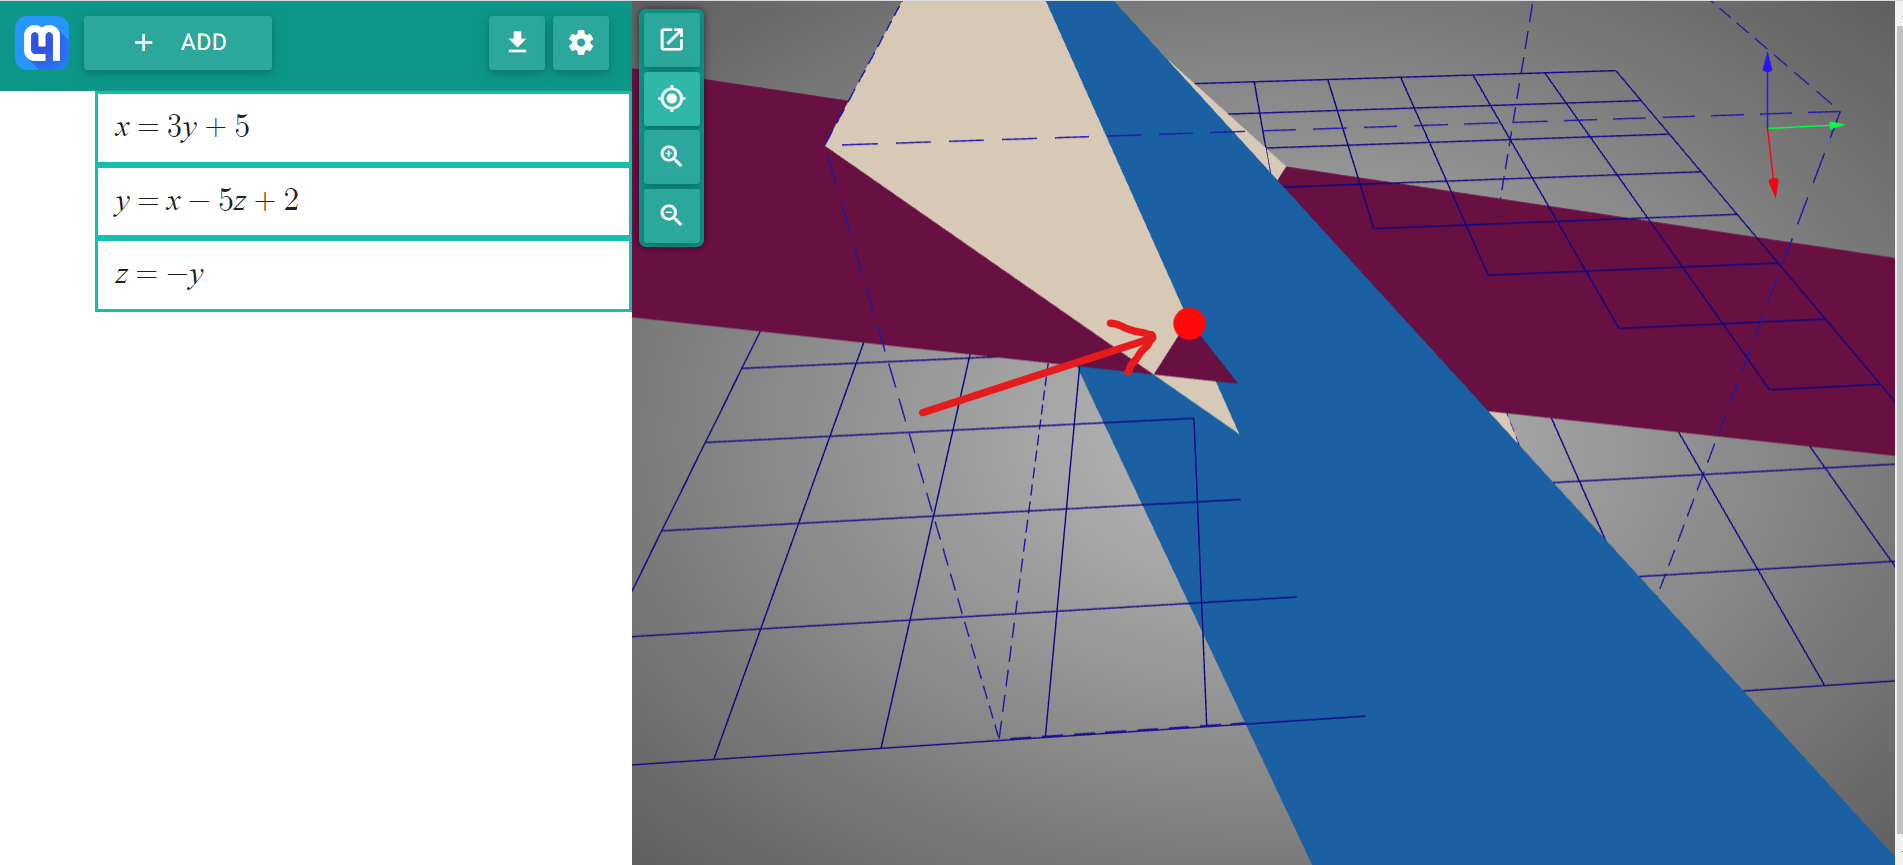
\includegraphics[width=0.85\textwidth]{system1}
	      		\caption{The first system}
	      		\label{fig:system1}
	      \end{figure}
	\item Second system:
	      \begin{equation*}
	      	\begin{cases}	
	      		2x_1+x_2+4x_3=-1 \\
	      		x_1+x_2+x_3=-1   \\
	      		x_1-x_2+5x_3=1   
	      	\end{cases}
	      \end{equation*}
	      Present the system as arguemented matrix $ \left[ A|b \right] $ :
	      \begin{equation*}
	      	\begin{bmatrix}
	      		2 & 1  & 4 & -1 \\
	      		1 & 1  & 1 & -1 \\
	      		1 & -1 & 5 & 1  
	      	\end{bmatrix}
	      \end{equation*}
	      Then, do some elementary transformations to make row-echelon form:
	      \begin{equation*}
	      	\begin{split}
	      		& \begin{bmatrix}
	      		2 & 1 & 4 & -1 \\
	      		1 & 1 & 1 & -1 \\
	      		1 & -1 & 5 & 1
	      		\end{bmatrix}
	      		(\RomanNumeralCaps{1}) \leadsto
	      		\begin{bmatrix}
	      			1 & 1  & 1 & -1 \\
	      			1 & -1 & 5 & 1  \\
	      			2 & 1  & 4 & -1 
	      		\end{bmatrix}
	      		(\RomanNumeralCaps{2}) \leadsto \\
	      		&(\RomanNumeralCaps{2}) \leadsto
				\begin{bmatrix}
	      			1 & 1  & 1 & -1 \\
	      			0 & -2 & 4 & 2  \\
	      			0 & -1 & 2 & 1  
	      		\end{bmatrix}
	      		(\RomanNumeralCaps{3}) \leadsto
	      		\begin{bmatrix}
	      			1 & 1  & 1 & -1 \\
	      			0 & -2 & 4 & 2  \\
	      			0 & 0  & 0 & 0  
	      		\end{bmatrix}
	      	\end{split}
	      \end{equation*}
	      (\RomanNumeralCaps{1}) Swap the rows to easier reach the row-echelon form \\
	      (\RomanNumeralCaps{2}) Subtract $R_1$ from $R_2$, subtract $2R_1$ from $R_3$ \\
	      (\RomanNumeralCaps{3})	Add $R_2$ divided by -2 to $R_3$ \\\\
	      As we can see the ruslt matrix has the zero line that means $x_3$ is a free variable and the system has an infinity 				number of solutions.\\
		\newpage
	      In the figure \ref{fig:system2_org}, the \textit{intersection} of three planes is the solution of 				the system, in this case it is a \textit{straight line}, so the number of solutions \textit{is infinite}. In the figure \ref{fig:system2_con}, we see that there are 				only 2 planes left, but the solution of the system is the same straight line.
		 \vspace{1cm}
	      \begin{figure}[H]
	      		\centering
	      		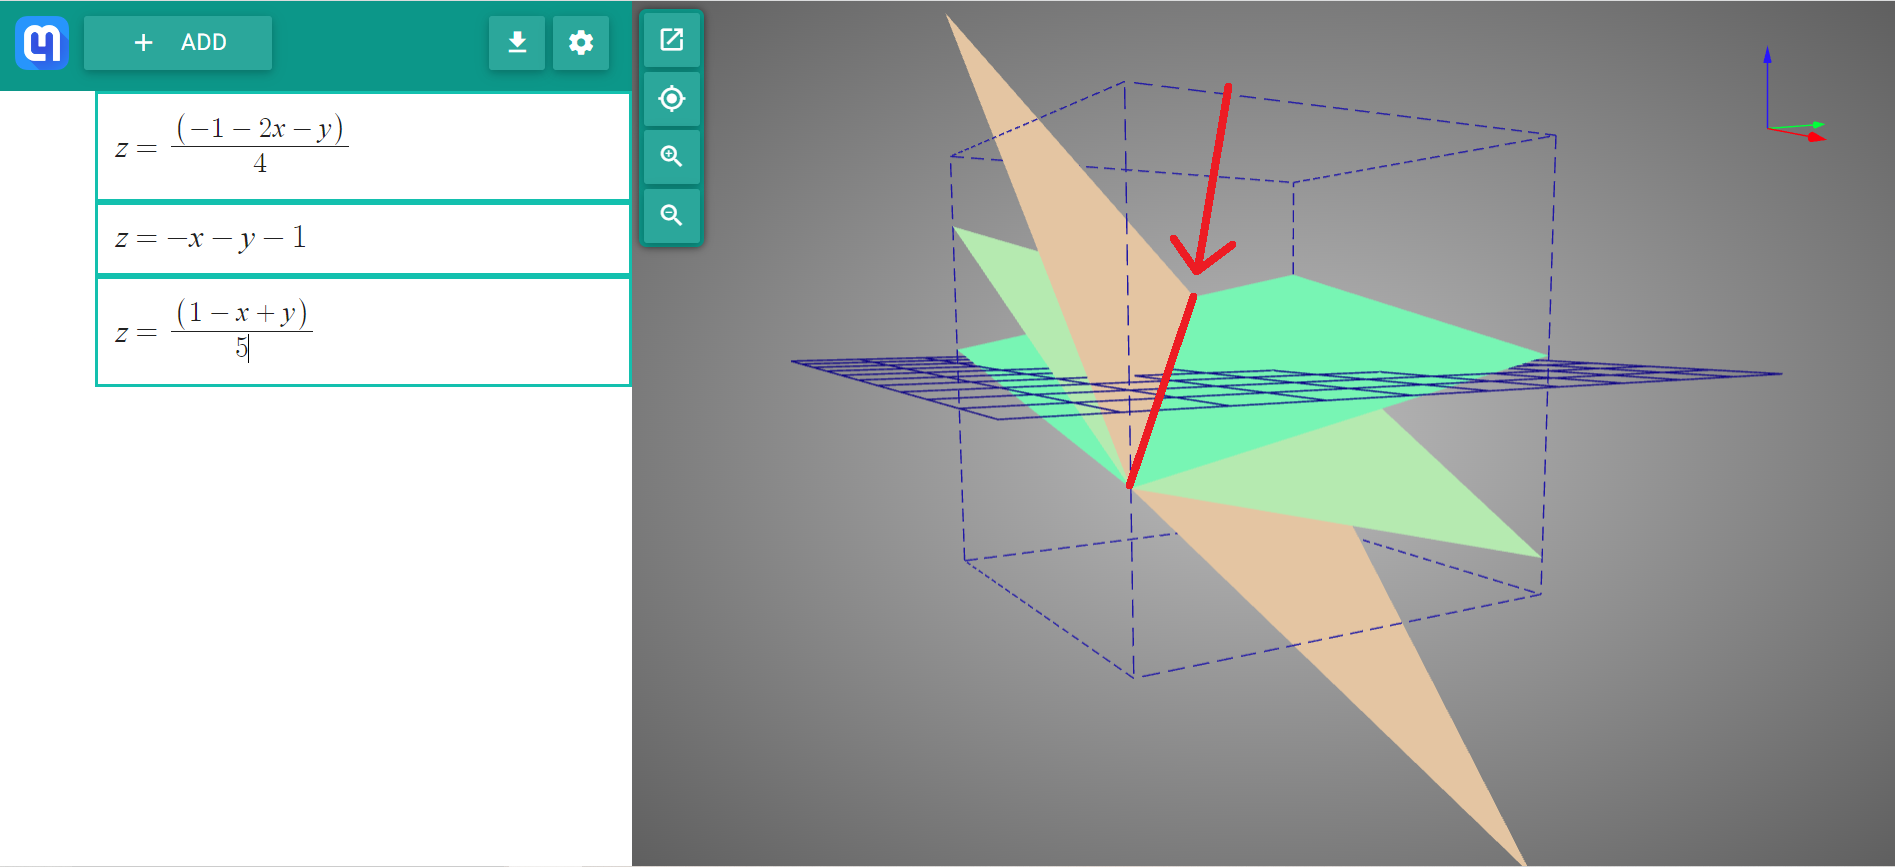
\includegraphics[width=0.85\textwidth]{system2_normal}
	      		\caption{The original system}
	      		\label{fig:system2_org}
		\end{figure}
		 \vspace{1cm}
		\begin{figure}[H]
	      		\centering
	      		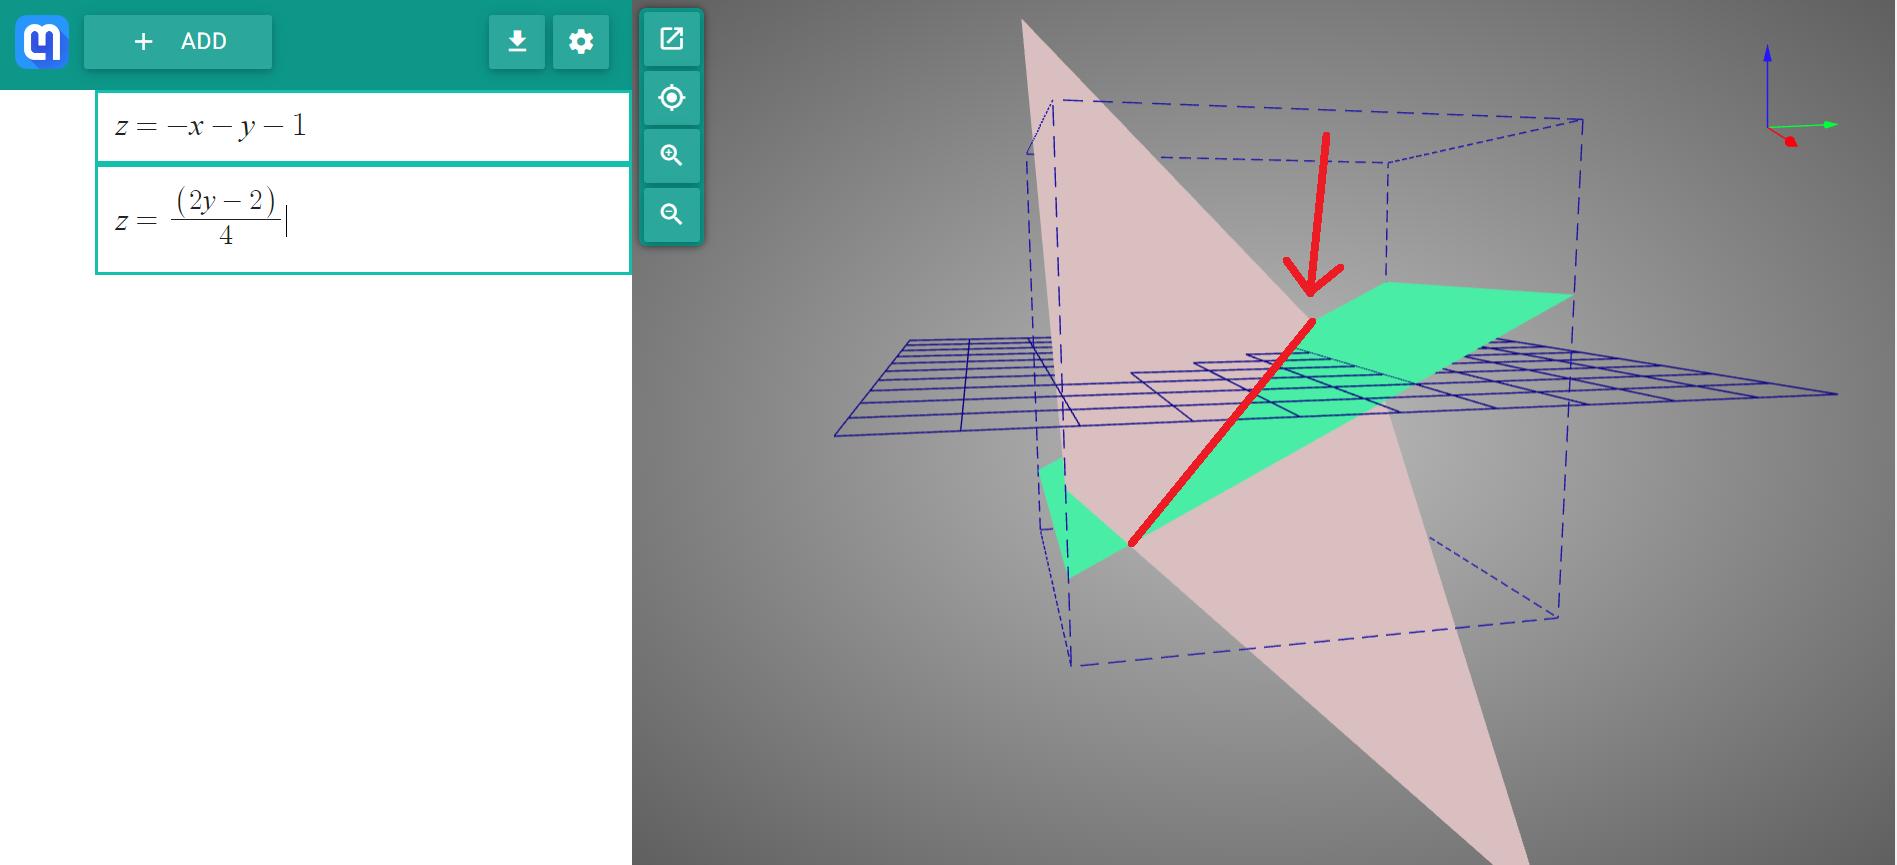
\includegraphics[width=0.85\textwidth]{system2_converted}
	      		\caption{The converted system}
	      		\centering
	      		\label{fig:system2_con}	
	      \end{figure}
	\newpage
	\item Third system:
		\begin{equation*}
	      	\begin{cases}	
	      		x_1+x_3=1 \\
	      		-x_1+x_2=0 \\
	      		x_2+x_3=0
	      	\end{cases}
	      \end{equation*}
		Present the system as arguemented matrix $ \left[ A|b \right] $ :
	      \begin{equation*}
	      	\begin{bmatrix}
	      		1 & 0  & 1 & 1 \\
	      		-1 & 1  & 0 & 0 \\
	      		0 & 1 & 1 & 0  
	      	\end{bmatrix}
	      \end{equation*}
		Then, do some elementary transformations to make row-echelon form:
		\begin{equation*}
	      	\begin{split}
	      		\begin{bmatrix}
		      		1 & 0  & 1 & 1 \\
		      		-1 & 1  & 0 & 0 \\
		      		0 & 1 & 1 & 0
	      		\end{bmatrix}
	      		(\RomanNumeralCaps{1}) \leadsto
	      		\begin{bmatrix}
		      		1 & 0  & 1 & 1 \\
		      		0 & 1  & 1 & 1 \\
		      		0 & 1 & 1 & 0
	      		\end{bmatrix}
	      		(\RomanNumeralCaps{2}) \leadsto
	      		\begin{bmatrix}
		      		1 & 0  & 1 & 1 \\
		      		0 & 1  & 1 & 1 \\
		      		0 & 0 & 0 & -1
	      		\end{bmatrix}
	      	\end{split}
	      \end{equation*}
	      (\RomanNumeralCaps{1}) Add $R_1$ to $R_2$ \\
	      (\RomanNumeralCaps{2}) Subtract $R_2$ from $R_3$ \\\\
		In the third row we get impossible equality --- $0 = -1$, so this system \textit{doesn't have solution}.\\
		As you see, there is \textit{no intersection} of three plane in one point/line in the figure \ref{fig:system3}.
		\begin{figure}[H]
      		\centering
      		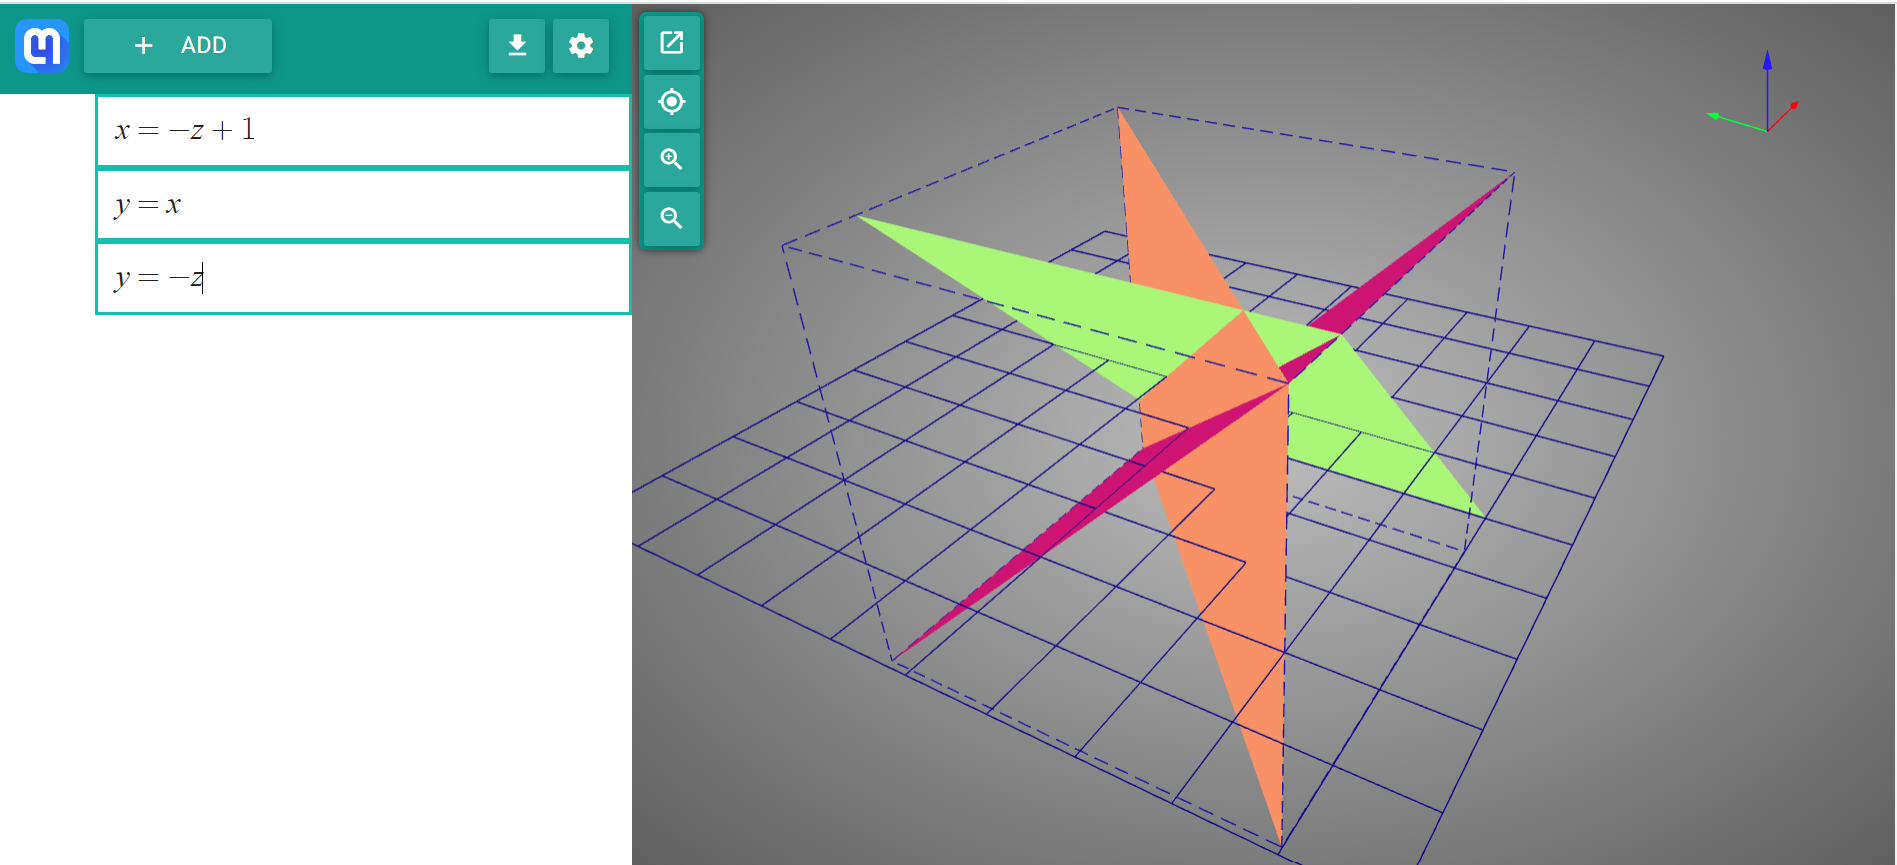
\includegraphics[width=0.85\textwidth]{system3}
      		\caption{The third system}
      		\label{fig:system3}
	      \end{figure}
\end{enumerate}
\end{document} 